\chapter{Inhalt von Notfallrucksack/Sauerstofftasche/Schienentasche}
\section{Notfallrucksack}
Der Rucksack besteht aus einem großen "Hauptraum" sowie 2 Taschen an der Vorderseite.
Im Hauptraum sind an den beiden Seiten jeweils Taschen mit Klettverschluss befestigt.
\subsection*{Seite A}
\begin{figure}[H]
    \centering
    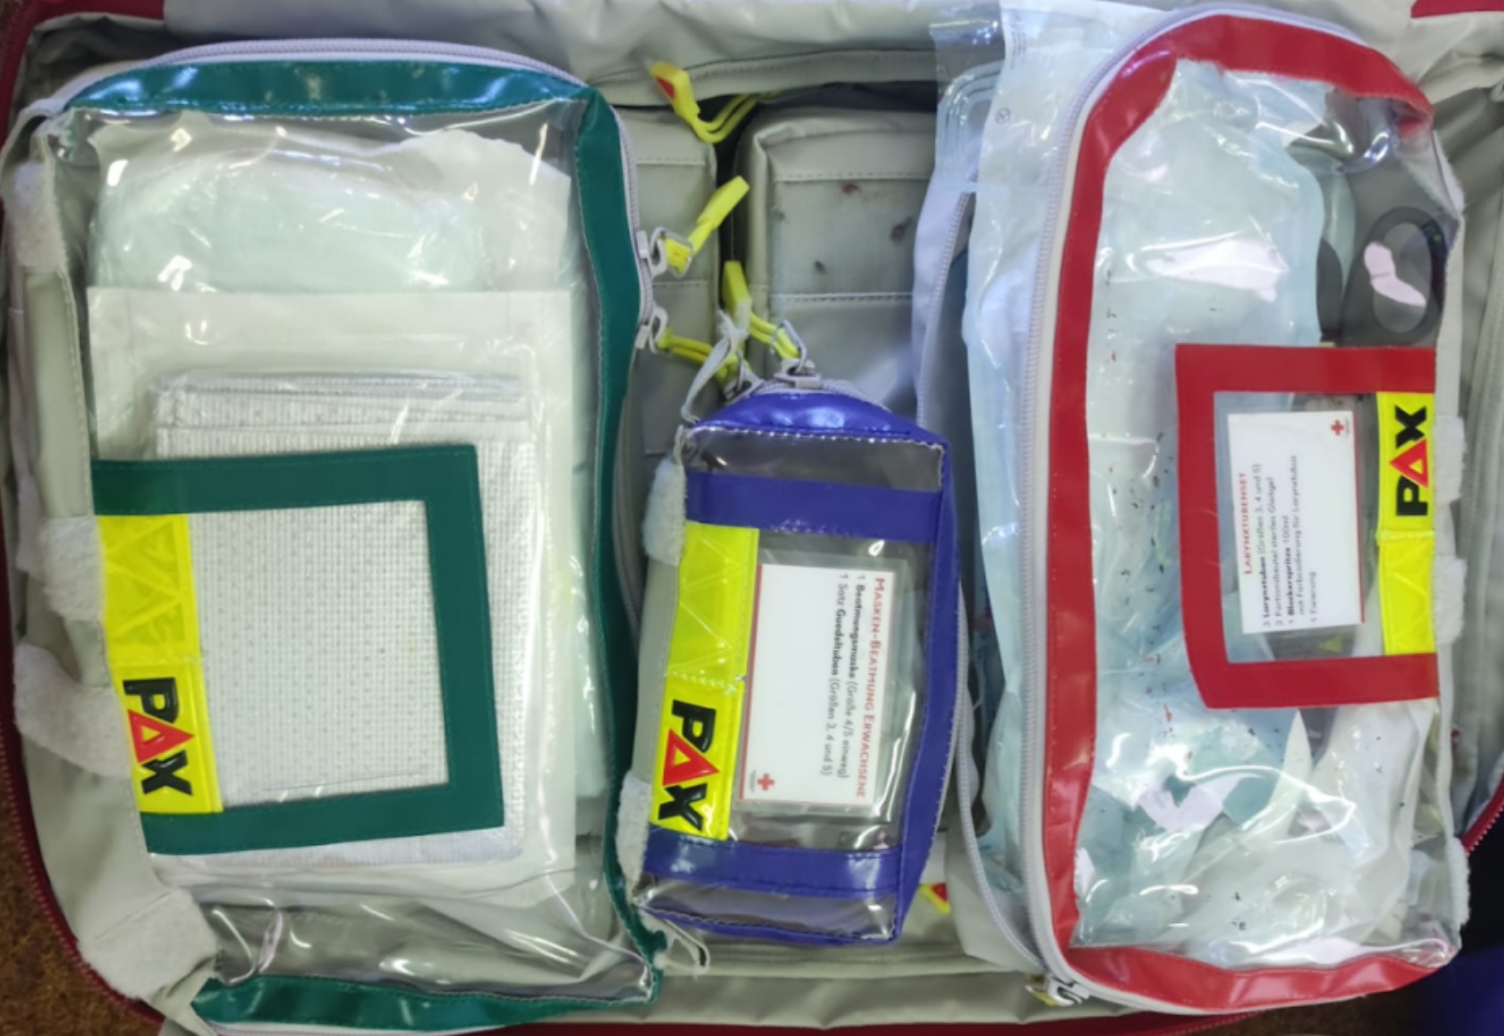
\includegraphics[width=\textwidth]{res/rucksack_a.png}
\end{figure}
\begin{itemize}
    \item Rote Tasche: Larynx Tubus (in 3 Größen) inkl. Zubehör (Blockerspritze, Gleitgel, Etwas zum Fixieren)
    \item (Kleine) blaue Tasche: Guedel Tubus (in 3 Größen)
    \item Grüne Tasche: Wundauflagen (saugende/metallische) \& Verbandmaterial
\end{itemize}
\subsection*{Seite B}
\begin{figure}[H]
    \centering
    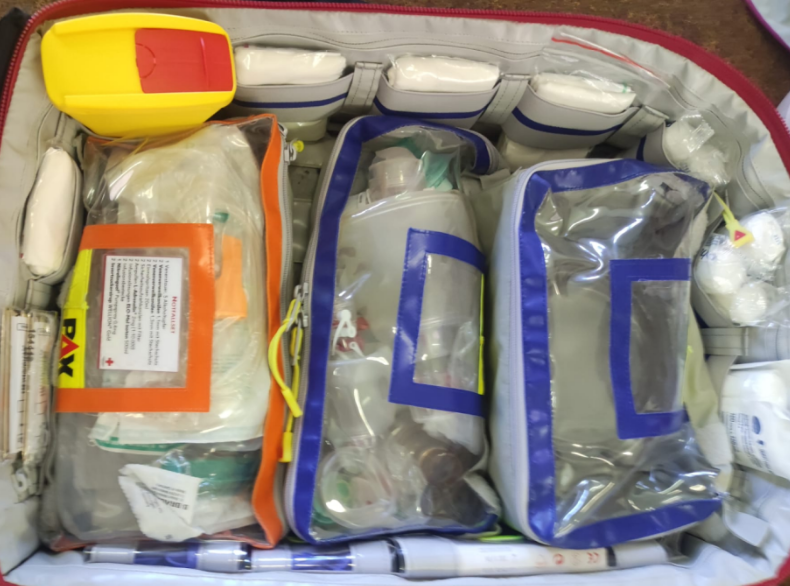
\includegraphics[width=\textwidth]{res/rucksack_b.png}
\end{figure}
\begin{itemize}
    \item Blaue Taschen: Beatmungsbeutel inkl. Zubehör (Luftfilter\dots)
    \begin{itemize}
        \item Je eine Tasche für Erwachsene und Kinder + Säuglinge
    \end{itemize}
    \item Orange Tasche: Material für venösen Zugang / Infusionen
    \item Am Rand: Contamed-Box (Stichfester Behälter für Nadeln etc.), Mullbinden, Wärmedecken, Dreickstücher, Handschuhe
\end{itemize}

\subsection*{Vorderseite Oben - Diagnostik}
\begin{figure}[H]
    \centering
    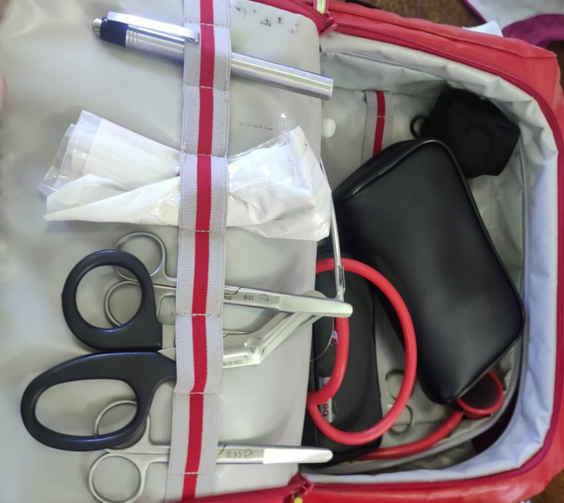
\includegraphics[scale=.5]{res/rucksack_vorne_oben.png}
\end{figure}
\begin{itemize}
   \item Pupillenlampe
   \item Eigentumsbeutel
   \item Scheren
   \item Stethoskop
   \item Pulsoximeter 
   \item Blutzuckermessgerät
   \item Defibrillator 
\end{itemize}

\subsection*{Vorderseite Unten}
\begin{figure}[H]
    \centering
    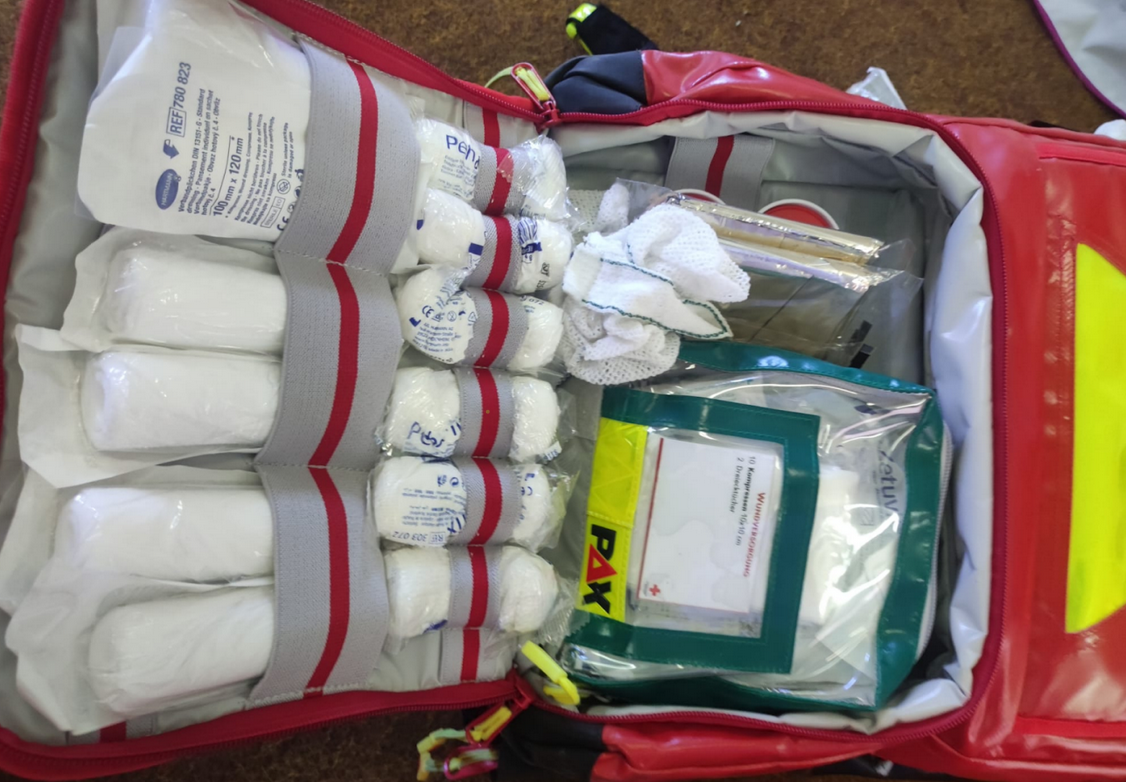
\includegraphics[scale=.5]{res/rucksack_vorne_unten.png}
\end{figure}
\begin{itemize}
   \item Mullbinden
   \item Kompressen
   \item Momentverband (=Mullbinde mit integrierter Wundauflage)
   \item Dreieckstücher
   \item Wärmedecken
   \item Kopfhaube
   \item Leukoplast 
\end{itemize}

\section{Sauerstofftasche}
\begin{figure}[H]
    \centering
    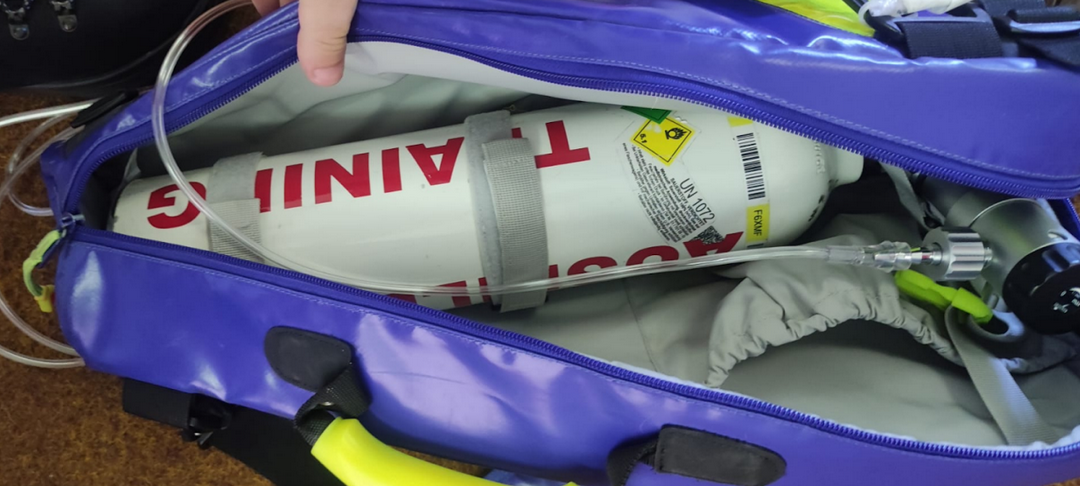
\includegraphics[scale=.5]{res/sauerstofftasche.png}
\end{figure}
\begin{itemize}
    \item Sauerstoffflasche mit Druckminderer
    \item Atemmaske
    \item Nasenbrille
    \item Schlauch
    \item Vor Dienstbeginn kontrollieren, ob genügend Druck vorhanden ist!
\end{itemize}

\section{Schienentasche}
\begin{itemize}
    \item Stiffnecks
    \item Sam Splints (für Unterarm/Knöchel)
    \item Unterschenkel-Vakuum-Schiene
\end{itemize}